
\section{Introduction}
\label{sec:introduction}

In this paper, we investigate \emph{tiebreaking strategies} for cost-optimal \astar.
% In optimal search, tiebreaking strategies does not affect the optimality
% of the search algorithms because they only affect the node expansion
% order among the nodes with the same $f$-cost.
% \subsection{Tiebreaking for \astar}
% This paper is organized as follows.
% After defining some notations in \refsec{sec:preliminaries}, 
% We first investigate the conventional
% tiebreaking strategies for the optimal search using \astar.
\astar is the standard search
algorithm for finding an optimal-cost path from an initial state $s$ to
some goal state $g \in G$ in a search space represented as a graph
\cite{hart1968formal}.
In many problems, the size of the last layer of the search, called
\emph{final plateau}, accounts for a significant fraction of the
effective search space of \astar.  \refig{fig:plateau-noh}
(\refpage{fig:plateau-noh}) plots the number of states with $f(n) = f^*$
(y-axis) vs. the number of states with $f(n) \leq f^*$ for 1104 problem
instances from the International Planning Competition (IPC1998-2011),
where $f^*$ is the optimal cost and $f(n)$ is a lower bound of the cost of the shortest path
that contains a node $n$.  For many instances, a large
fraction of the nodes in the effective search space have $f(n)=f^*$:
The points are located very close to the diagonal line
($x=y$), indicating almost all states with $f(n) \leq f^*$ have cost $f^*$.
This is depicted in \refig{fig:plateau-0}. 
A naive view of the search space would consider the search space of \astar as a region with a thin layer representing the  final plateau surrounding a large number of closed nodes with $f<f^*$ (left).
% Note that this naive view accurately describes some real, practical search spaces, e.g., 2D path finding on an explicit graph.
However, for many combinatorial search problems, 
% due to the curse of dimensionality, %``curse of dimensionality'' 
the figure on the right is a more accurate depiction -- the  search space has a large plateau 
for $f=f^*$.\todo{The fact that the last layer of search dominates the search was the motivation for Frontier Search and its numerous variants, so the SoCS community has been well aware of this}

\begin{figure}[htbp]
  \centering
  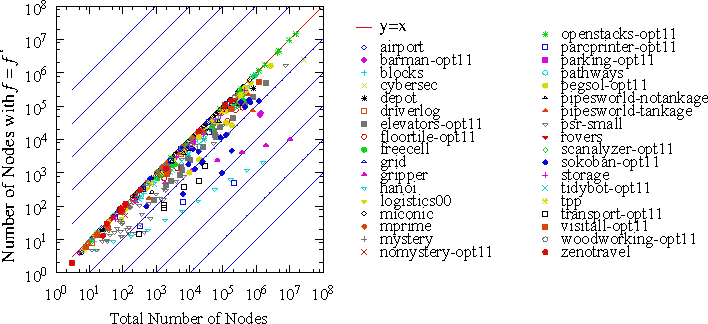
\includegraphics{tables/aaai16-frontier/aaai16prelim3/lmcut_frontier_noh-front.pdf}
 \caption{
 The number of nodes with $f=f^*$ (y-axis) compared to the
 total number of nodes in the search space (x-axis) with $f\leq f^*$ on 1104 IPC benchmark problems,
  using modified Fast Downward with \lmcut which 
  generates all nodes with cost $f^*$.
  }
 \label{fig:plateau-noh}
\end{figure}

\begin{figure}[htbp]
  \centering
  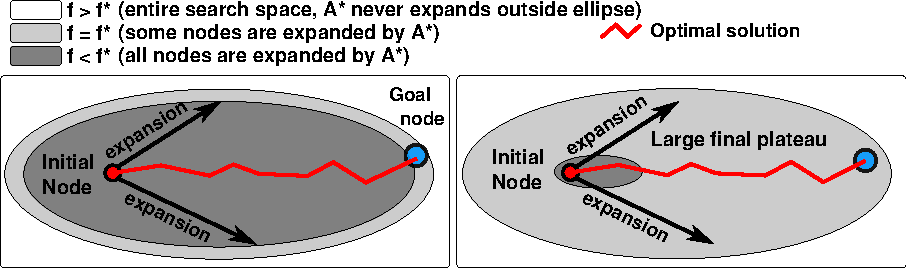
\includegraphics{img/astar/plateau-0.pdf}
 \caption{(Left) Naive and incorrect understanding of the search space. (Right) In reality, plateau containing the optimal goals ($f=f^*$) is large, and it even accounts for most of the search effort required by \astar.
  }
 \label{fig:plateau-0}
\end{figure}

Therefore, in the majority of IPC problem domains, where the 
the last layer ($f(n)=f^*$) accounts for a significant fraction of the effective search space, a
\emph{tiebreaking strategy} which determines which node to 
 expand among nodes with the same $f$-cost,
can have a significant impact on the
performance of \astar. 
It is widely believed that among nodes with the same $f$-cost,
ties should be broken according to $h(n)$, i.e.,
nodes with smaller $h$-values should be expanded first.  While this is a
useful rule of thumb in many domains, it turns out that tiebreaking
requires more careful consideration, particularly for problems where
most or all of the nodes in the last layer have the same $h$-value.

We empirically evaluate the existing, commonly used, standard
tiebreaking strategies for \astar (\refsec{sec:eval-common-strategies}).
We show that:

\begin{enumerate}
 \item A Last-In-First-Out (\lifo) criterion tends to be more efficient
       than a First-In-First-Out (\fifo) criterion.
 \item Tiebreaking according to the heuristic value $h$, which
       frequently appears in the heuristic search literature, has little
       impact on the performance as long as \lifo default criterion is used 
       --  in other words, a \lifo tiebreaking policy is sufficient for most IPC domains.
 \item There are significant performance differences among tiebreaking strategies
       when domains include zero-cost actions. This is true even when $h$-based tiebreaking is used.
\end{enumerate}

While there are relatively few domains with zero-cost actions in the IPC
benchmark set, we argue that zero-cost actions naturally occur in
practical cost-minimization problems. Therefore we introduce a new set of
benchmarks called \emph{zerocost domains}
(\refsec{sec:zerocost-domains}).  We empirically show that these
zerocost domains have the different search space structure and different
problem difficulty from those of the original domains.

In order to solve such problems more efficiently, we propose and
evaluate \emph{depth diversification}, a new
tiebreaking method based on the notion of a node's \emph{depth} within a plateau,
which corresponds to the number of steps from the ``entrance'' to
the plateau (\refsec{sec:depth},
\refsec{sec:depth-based-evaluation}). We also propose and evaluate an
admissible method which uses the distance-to-go estimate, an estimate which treats every actions
to have the unit costs (\refsec{sec:distance-to-go}).
In these sections, we empirically show that:
\begin{enumerate}
 \item Our new depth-based diversification strategy significantly improves upon the 
       existing tiebreaking strategies using the same heuristic function.
 \item \emph{Inadmissible} distance-to-go variations of \emph{admissible} heuristics
       (\lmcut, \mands)
       significantly outperforms the tiebreaking using the original admissible heuristics.\todo{listing 3 points regarding d2go might give the wrong impression that this paper is about d2go. combine some of the d2go bullets, or add another depth-related bullet?}
 \item Distance-to-go variations of \emph{inadmissible} heuristics
       (\ff) further improves the performance by an order of magnitude.
 \item Distance-to-go variations of \emph{inadmissible} heuristics
       (\ff) combined with depth-based diversification further
       improves the performance.
\end{enumerate}

Finally, in \refsec{sec:discussion}, we discuss the implications of these
results. \todo{revise par based on what ends up remaining in the discussion section}
We offer a rather trivial, but new perspective to admissible
\astar search: \astar can be conceived as a sequence of independent runs
of satisficing Greedy Best First Search(GBFS)es in each plateau defined by the
$f$-value. We argue that arbitrary satisficing techniques improve the
search performance when applied as a tiebreaking strategy within
a plateau.
%  in the final plateau, which is the last and (usually) the largest
% layer of the search.
% 
Regressing from the new perspective, we also show a preliminary result
that the depth diversification tiebreaking, which has improved various
tiebreaking heuristics, also improves the performance of bare GBFS in
satisficing search.
We further discuss the future direction, related works, and close the article.

\textbf{
Note for reviewers:
This paper is a significantly extended version of the AAAI-16 paper by
the same authors. The addition to the conference paper is the following:
\begin{enumerate}
 \item Introduction of deterministic depth-based diversification
       strategy (as opposed to the randomized version in the conference
       paper), and its theoretical analysis in \refsec{sec:depth}. We
       also added thorough empirical analysis in
       \refsec{sec:depth-based-evaluation} that are not included in the
       conference version.
 \item Empirical analysis of distance-to-go estimates in
       \refsec{sec:distance-to-go}.  Also, we included an empirical
       evaluation of the use of inadmissible FF heuristics as part of
       tiebreaking criterion, and its combination with the
       depths metric thereof.
 \item New perspective to \astar and the preliminary results on the use
       of depth for satisficing planning (\refsec{sec:discussion}).
\end{enumerate}
}

